% XeLaTeX can use any Mac OS X font. See the setromanfont command below.
% Input to XeLaTeX is full Unicode, so Unicode characters can be typed directly into the source.

% The next lines tell TeXShop to typeset with xelatex, and to open and save the source with Unicode encoding.

%!TEX TS-program = xelatex
%!TEX encoding = UTF-8 Unicode

\documentclass[10pt,a4paper,left=15mm,right=15mm,top=20mm,bottom=20mm]{article}
\usepackage{geometry}                % See geometry.pdf to learn the layout options. There are lots.
\usepackage[hangul]{kotex}
\usepackage{indentfirst}
\geometry{letterpaper}                   % ... or a4paper or a5paper or ... 
%\geometry{landscape}                % Activate for for rotated page geometry
%\usepackage[parfill]{parskip}    % Activate to begin paragraphs with an empty line rather than an indent
\usepackage{graphicx}
\DeclareGraphicsExtensions{.pdf,.png,.jpg,.jpeg}
\usepackage{amssymb}

% Will Robertson's fontspec.sty can be used to simplify font choices.
% To experiment, open /Applications/Font Book to examine the fonts provided on Mac OS X,
% and change "Hoefler Text" to any of these choices.

\usepackage{fontspec,xltxtra,xunicode}
\defaultfontfeatures{Mapping=tex-text}
\setmainhangulfont{Sarasa Mono K Nerd Font Complete}
\setromanfont[Mapping=tex-text]{Sarasa Mono K Nerd Font Complete}
\setsansfont[Scale=MatchLowercase,Mapping=tex-text]{Sarasa Mono K Nerd Font Complete}
\setmonofont[Scale=MatchLowercase]{D2Coding}

\title{Alcor}
\author{snowmerak}
%\date{}                                           % Activate to display a given date or no date

\begin{document}
\maketitle

\tableofcontents
\listoffigures

\newpage
\section{서론}

\subsection{배경}

투표는 대의제 민주주의에 있어 매우 중요한 권리 행사와 의사 표명의 수단이다. 하지만 기존의 종이 투표는 한번 시행할 때 투표 용지부터 장소 대여, 관련 비품 구입, 관련 인력 채용, 투표 용지 확인 및 검산, 그리고 참관인까지 매우 많은 비용이 들어가게 된다. 게다가 언제 가능할지 모르는 유권자를 위해 투표 시간을 길게 잡아야 하고 물리적으로 정상적인 투표가 불가능할 경우 사전 투표를 따로 시행해야한다.

그리고 시장에 나와 있는 블록체인 투표 앱은 서버에 블록체인 형태로 저장하는 방식을 쓰는 경우가 있는데 이 경우엔 유권자 입장에서 제대로 등록 되었는지, 그렇지 않은지 알 수 없는 경우가 많았으며 반대로 퍼블릭 블록체인을 사용하게 될 경우에는 누구나 투표 과정을 알 수 있지만 합의에 의해 투표 시간이 계속해서 늘어져서 정상적인 진행을 못 할 수도 있다.

그래서 투표가 오래 걸리지 않고 누구도 함부로 조작할 수 없게 저장하여 누구나 어렵지 않게 투표 과정을 확인하고 로컬에서 검산할 수 있는 서비스를 만들기로 하였다.

\subsection{목표 및 수단}

이 과제의 목표는 크게 3 가지이다.
\begin{enumerate}
 \item 투표 시간이 오래 걸리지 않을 것, 즉 고성능일 것.
 \item 함부로 수정할 수 없는 데이터 구조를 가질 것.
 \item 누구나 어렵지 않게 투표 결과를 감시할 수 있을 것.
\end{enumerate}

고성능을 만들어 내기 위해 우리가 고려한 부분은 저비용과 동시성이다. 최대한 네트워크 통신 비용을 최소화하고 서버에서 제공하는 API 기능도 최대한 작은 단위로 분리하여 하나하나의 응답 시간을 최소화하고 한번에 많이 처리하는 것을 우선적으로 고려하였다. 각 세션을 유지하기 위해 서버가 부담해야할 메모리 비용은 커지겠지만 각 요청과 응답의 처리 비용은 줄어들 것으로 기대된다.

조작 불가능한 데이터 구조를 만들기 위해 고려한 것은 블록체인이다. 블록체인은 각 블록이 이전 블록의 해시에 의존성을 가짐으로 이전 블록과 이후 블록의 수정이 없으면 현재 블록의 수정 또한 거의 불가능해지는 구조를 가진다. 하지만 블록체인은 특수한 형태가 아닌 이상 싱글 스레드처럼 움직이게 되고 이 형태는 결과적으로 동시성에 가장 큰 방해물이 된다.

그래서 우리는 비트코인과 마찬가지로 실제 투표 용지 여러개를 묶어서 하나의 번들을 만든 후 이 번들을 블록으로 사용하는 방법을 차용하였다. 이 번들을 채우는 여러개의 투표 용지는 비동기로 처리된 요청들이 하나의 버퍼에 담기게 되고 일정 수가 충족되면 하나의 번들에 담겨서 체인 형태로 기록된다. 이렇게 되면 실제 락에 의해 정지되는 일순간과 버퍼를 비우고 등록하는 짧은 시간을 제외하면 비동기적으로 투표를 처리하는 것이 가능하게 된다.

그리고 블록체인과 마찬가지로 타원 곡선 전자 서명 알고리즘을 활용하여 투표 용지를 검증할 수 있다. 일련의 과정은 블록체인과 동일하게 클라이언트에서 만든 키페어 중에서 공개키만 서버에 전송하고 투표 과정 중 서버는 공개키를 이용하여 검증을 한번 거치고, 이후 투표가 종료되면 모두에게 공개되어 누구나 투표 용지가 조작되지 않았는 지 검증할 수 있다.

마지막으로 누구나 어렵지 않게 투표 결과를 감시할 수 있게 하기 위해 서버에서 투표 용지와 유권자의 공개키, 번들 정보를 공개하는 API를 제공하여 별도의 클라이언트 프로그램을 통해 그래픽 유저 인터페이스를 이용하여 투표 과정과 결과를 감시할 수 있다. 이 클라이언트도 옵저버라는 이름으로 같이 제공할 것이다.

\section{본론}

\subsection{개발 내용}

\subsubsection{서버 API 구조}

\begin{figure}[h]
    \begin{center}
        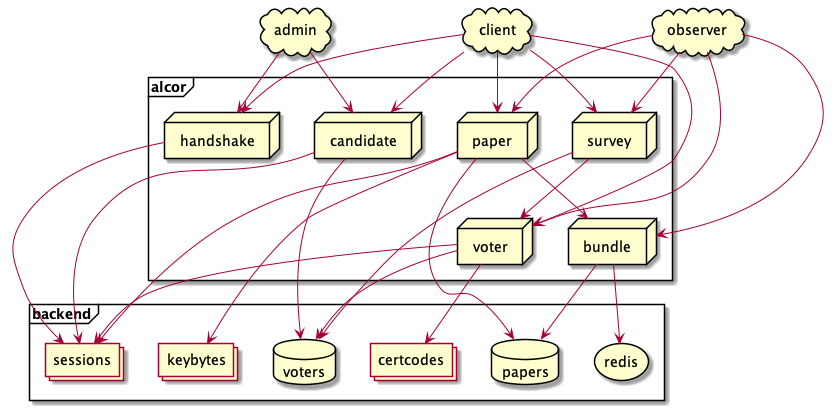
\includegraphics[width=13cm]{server}
        \caption{서버 API 구조}
    \end{center}
\end{figure}

그림 1은 서버의 대략적인 구성을 그린 다이어그램이다. 서버는 총 6개의 레스트풀 API를 제공한다.

\begin{enumerate}
    \item handshake
    
    이 과제의 서버는 2가지 이유로 TLS를 사용하지 않는다. 하나는 웹 브라우저가 아니라 클라이언트를 제공할 것이기 때문에 직접 키교환을 통해 대칭키를 만들어 사용하는 것이 더 비용 측면에서 저렴하다고 판단하였으며, 다른 하나는 신뢰할 수 있는 인증서 발급 과정을 생략하여 초기 설정을 간소화할 수 있기때문이다.

    그래서 키교환을 수행할 수 있게 해당 API가 필요하다. 관리자(admin)와 유권자(client)는 이 API를 통해 서버와 키교환을 수행하고 세션을 할당받게 된다. 서버는 이 세션을 메모리 캐시에 저장하게 된다.
    
    세션은 오래 접근하지 않은 데이터를 우선적으로 삭제하고 디스크에 백업될 필요가 없으며 다른 라우트에서도 동시에 접근할 수 있도록 하기 위해 맴캐시드를 사용한다.

    \item voter
    
    이 API는 유권자 정보를 관리하게 된다. 유권자(client)는 이 API를 통해 본인인증을 하고 미리 약속한 타원 곡선 디지털 서명 알고리즘에 의해 만들어진 자신의 공개키를 제공하고 투표를 위한 익명 아이디를 받는다.

    본인인증 과정은 기본 값으로 휴대폰 본인인증을 우선적으로 지원할 것으로 유권자가 요청한 휴대폰 인증 번호를 저장할 메모리 캐시가 필요하다. 이 메모리 캐시 또한 세션과 마찬가지로 디스크에 백업될 필요가 없기 때문에 멤캐시드를 사용하였다.

    마지막으로 유권자가 보낸 공개키와 서버가 제공한 아이디는 서버의 voters 데이터베이스에 저장한다.

    \item paper
    
    이 API는 유권자에게는 투표 절차를 제공하고 참관인(observer)에게는 투표 결과를 제공한다. 투표를 위해 유권자는 먼저 투표를 이 API에 투표를 요청하게 된다. 그러면 서버는 임의로 만들어진 바이트 버퍼를 유권자에게 제공하고 유권자는 이 바이트 버퍼를 포함하여 자신의 아이디, 후보 이름, 투표 시간을 기록하고 미리 약속된 해시 알고리즘에 따라 해싱한 후 그 출력 값을 서명하여 이것, 투표지를 서버에 전송한다.

    서버는 미리 제공한 임의의 바이트 버퍼를 keybytes라는 메모리 캐시에 저장하고 있다가 유권자가 투표지를 보내오면 그 바이트 버퍼를 확인한다. 이 과정은 이후에라도 혹시 모를 유권자의 해시 값 조작을 어렵게 하기 위한 장치이다.

    임의의 바이트 버퍼 값이 동일함을 확인한 서버는 투표지의 값을 기반으로 다시 해시 값을 만들어 올바른 해시 값인지 확인하고 미리 받아 놓은 공개키를 통해 서명이 올바른지 검증한 후 papers 데이터베이스에 저장한다.

    그리고 이 투표지의 해시 값은 bundle API에 전달하여 블록체인 구조를 만드는 과정에 사용된다.

    \item bundle
    
    이 API는 외부적으로 참관인만이 접근할 수 있다. 참관인은 이 API를 통하여 현재 마지막으로 등록된 번들의 해시 값을 받아올 수 있다. 번들 객체는 일정 수의 투표지 해시 값과 이전 번들의 해시 값으로 이루어져 있고 이 값을 통해 거꾸로 올라가는 방식으로 모든 블록체인 구조를 순회할 수 있다.

    순회하면서 당연히 번들에 묶인 투표지 해시 값을 통해 각 투표지에 접근할 수 있으며 이는 paper API를 통해 얻을 수 있다. 그리고 투표지 객체 내에서 유권자 아이디를 통해 해당 투표지를 제출한 유권자의 공개키를 voter API를 통해 요구할 수 있고 결과적으로 참관인은 후보와 서버의 휘발성 데이터를 제외한 모든 것을 얻을 수 있다.

    또한 이 API는 투표지 해시 값을 받아올 때 동시성을 넘어 병렬적으로 움직여야하는데 이를 위해 내부적으로 락프리 알고리즘에 버금가는 것을 구현해야한다.

    \item candidate
    
    이 API는 유권자가 투표할 후보를 등록하고 조회한다. 후보는 이름과 간단한 자기 소개나 공약을 작성한 마크다운 문서로 이루어져 있다.
    
    관리자가 후보를 등록하면 voters 데이터베이스에 등록하게 된다. 이는 후보만을 저장하는 데이터베이스를 분리하기엔 후보 수가 유권자나 투표 용지에 비해 지나치게 적다는 것과 투표 용지를 기록하는 papers 데이터베이스에는 bundle 객체도 담아야하기 때문에 부하를 맞추기 위함이다.

    \item survey
    
    이 API는 유권자가 투표를 마치고 간단한 설문조사를 작성하고 제출한다. 해당 선물조사는 voters 데이터베이스에 등록되고 참관인이 조회할 수 있으며 간단한 통계와 시각화 또한 제공할 것이다.

\end{enumerate}

\subsection{서버 투표 기능 구현}

    \subsubsection{서버 구현 도구}

    서버는 동시성에 강점을 보이고 네이티브로 컴파일 되어 성능적 강점 또한 얻을 수 있는 고 언어로 선택하였다. 고 언어는 그린 스레드보다 하위에 더욱 가벼운 고루틴 레이어를 두고 있어서 하나의 연결을 더욱 가볍게 처리할 수 있다. 그리고 언어 자체가 간결하고 쉽기 때문에 누구나 쉽게 배울 수 있으며 확장하기에도 편리하다.

    \subsubsection{핸드셰이크}

    \begin{figure}[h]
        \begin{center}
            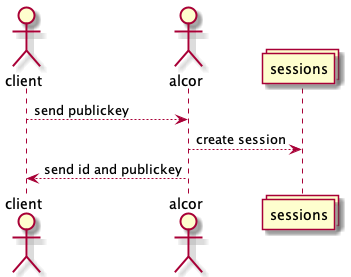
\includegraphics[width=8cm]{handshake}
            \caption{핸드셰이크 시퀸스 다이어그램}
        \end{center}
    \end{figure}

    클라이언트는 타원 곡선 키교환 알고리즘인 X25519에 의해 생성된 공개키를 서버에게 제공한다. 서버는 클라이언트의 요청이 들어오면 동일하게 X25519를 이용하여 개인키와 공개키를 생성하고 클라이언트의 공개키를 통해 대칭키를 생성한다. 서버는 이 대칭키와 대칭키를 SHA256으로 해싱한 아이디를 동시에 sessions 멤캐시드에 저장한다. 여기까지 아무 에러도 없을 경우 서버는 OK 상태와 클라이언트가 사용할 아이디와 서버의 공개키를 제공한다.

    \subsubsection{캡슐}

    \begin{figure}[h]
        \begin{center}
            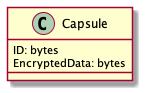
\includegraphics[width=3cm]{capsule}
            \caption{캡슐 클래스 다이어그램}
        \end{center}
    \end{figure}

    캡슐은 핸드셰이크로 얻은 대칭키로 데이터를 안전하게 암호화하여 통신하기 위한 구조체이다. ID는 세션 아이디이고 EncryptedData엔 아이디에 대응하는 대칭키로 암호화한 데이터가 포함된다. 이때 사용되는 데이터는 모두 프로토콜 버퍼(protobuf)로 만들어진다.

    프로토콜 버퍼를 사용한 이유는 Json보다 파싱이 빠르고 결과물도 더 가볍기 때문이다. 결과적으로 바이트 버퍼로 나오는 결과물은 암호화를 함에 있어 더욱 유용해진다. 그리고 암호화에는 AES256 기반의 갈루아/카운터 모드(GCM)을 활용하여 약간의 성능 향상과 안정성을 확보하였다.

    이 캡슐과 세션의 동작은 클라이언트가 캡슐을 암호화하고 서버에 전송한다. 서버는 캡슐을 받게되면 기록된 아이디를 기반으로 sessions에서 대칭키를 받아온다. 받아온 대칭키를 활용하여 캡슐 내용을 복호화하고 해당 서비스를 통해 작업을 수행한 후 결과는 다시 서버에서 암호화를 한 후 클라이언트에 전송한다. 클라이언트는 받은 캡슐을 복호화하여 데이터를 확인한다. 이 과정에 대한 시퀸스 다이어그램은 부록의 첫번째 그림인 <세션 시퀸스 다이어그램>에 올라가 있다.

    \subsubsection{유권자 등록}

    \begin{figure}[h]
        \begin{center}
            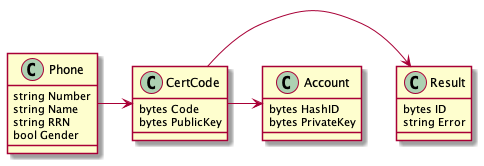
\includegraphics[width=12cm]{client-register-class}
            \caption{유권자 등록 클래스 다이어그램}
        \end{center}
    \end{figure}

    유권자 등록 다이어그램은 부록의 두번째 그림인 <유권자 등록 시퀸스 다이어그램>으로 삽입되어있다. 기본적으로 제공되는 방식은 휴대폰 본인 인증이다. 클라이언트는 휴대폰 번호와 필요한 개인정보를 담은 캡슐을 서버에 보낸다. 서버는 받은 데이터를 기반으로 이미 등록된 사람인지 확인한 후 휴대폰 본인 인증을 시도하고 certcodes에 인증 코드를 기록하고 OK 상태로 전송한다.

    클라이언트는 문자로 받은 인증 코드를 서버에 전송하고 서버는 certcodes에서 인증 코드를 가져와서 검증한다. 검증이 완료되면 OK 상태 메시지로 응답한다. 이때 클라이언트는 서버에 인증 코드와 동시에 타원 곡선 서명 알고리즘인 secp256r1을 기반으로 만들어진 공개키를 서버에 같이 전송하며 서버는 이 공개키를 기반으로 해싱하여 새로운 아이디를 만든 후 이 아이디와 공개키를 voters 데이터베이스에 저장한 후 클라이언트에 아이디를 추가로 전송한다.

    \subsubsection{후보 조회}

    \begin{figure}[h]
        \begin{center}
            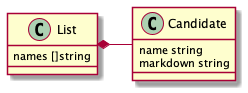
\includegraphics[width=7cm]{candidate-class}
            \caption{후보 클래스 다이어그램}
        \end{center}
    \end{figure}

    후보 조회 시퀸스 다이어그램은 부록의 <후보 시퀸스 다이어그램>으로 삽입되어있다. 후보 조회는 오로지 HTTP GET 요청으로만 이루어진다. 클라이언트는 /candidate 라우트에 GET 요청을 보내면 전체 후보 목록을 받을 수 있다. 후보 목록은 문자열 배열로 이루어진다.

    클라이언트는 이 후보 목록에서 후보 아이디를 선택하고 /candidate/:name 라우트에 GET 요청을 보내면 후보 이름에 해당하는 후보 정보를 받을 수 있다. 후보 정보는 이름과 후보에 대한 정보를 기록한 마크다운 문서로 이루어진다. 그리고 클라이언트에서는 이 마크다운 문서를 렌더링하여 유권자에게 후보에 대한 정보를 전달한다. 

    \subsubsection{투표}

    \begin{figure}[h]
        \begin{center}
            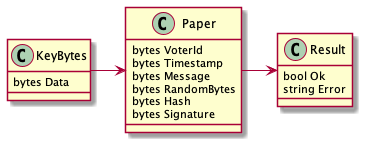
\includegraphics[width=10cm]{vote-class}
            \caption{투표 클래스 다이어그램}
        \end{center}
    \end{figure}

    투표 다이어그램은 부록 세번째 그림인 <투표 시퀸스 다이어그램>에 있다. 투표 또한 클라이언트 등록과 마찬가지로 크게 2개 부분으로 나뉘어진다. 첫번째는 클라이언트가 서버에 임의의 바이트 버퍼를 요구한다. 서버는 클라이언트에게 완전히 무작위로 생성된 바이트 버퍼를 제공한다. 이 바이트 버퍼는 crypto/rand 패키지의 함수를 사용하여 더욱 예측하기 어렵게 하고 이것은 해시 함수에 영향을 주기 위한 것으로 클라이언트가 해시를 조작할 수 있는 가능성을 고려하여 그 가능성을 어렵게 하기 위함이다. 그리고 이 바이트 버퍼는 keybytes에 저장하고 클라이언트에게 전송한다.

    두번째는 클라이언트가 받은 임의의 바이트 버퍼를 포함하여 자신의 유권자 아이디, 현재 시간, 메시지를 투표 용지에 저장한다. 그리고 이 투표 용지의 데이터들을 SHA256으로 해싱하여 저장한 후 개인키로 서명하여 서버에 전송한다. 서버는 keybytes에 요청하여 바이트 버퍼를 가져온다. 바이트 버퍼가 동일한지 확인하고 해시 또한 동일하게 연산되는 지 확인한다. 마지막으로 서버는 voters에서 유권자 정보를 받아서 서명을 검증하고 투표 용지를 papers 데이터베이스에 저장한다. 그리고 클라이언트에 투표 완료를 알린다.

    \subsubsection{번들링}

    \begin{figure}[h]
        \begin{center}
            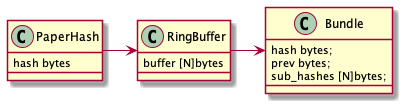
\includegraphics[width=10cm]{bundle}
            \caption{번들 클래스 다이어그램}
        \end{center}
    \end{figure}

    번들링의 시퀸스 다이어그램은 부록의 <번들 시퀸스 다이어그램>을 참고해주시기 바란다. 번들링은 투표 용지의 해시를 N개와 이전 해시를 모아 하나의 해시로 해싱하고 연관 해시를 포함하여 저장하는 것이다. 이를 통해 간단한 블록체인 형태의 데이터 구조를 구성할 수 있다. 그렇게 하기 위해 링버퍼의 동시성 처리는 Atomic Compare And Swap을 통해 뮤텍스 락보다 가볍게 처리하였다.

    Atomic Compare And Swap은 스레드에 영향을 받지 않는 atomic 연산을 통해 단일 변수에 대한 비교와 변경 연산을 동시에 수행하여 락 상태를 기록하는 것이다. 이 방식은 락프리(lock-free) 알고리즘은 아니지만 충분히 뮤텍스보다 빠르게 처리할 수 있다. 투표 요청이 끝난 후와 일정 수의 투표 용지 해시가 채워졌을 경우에도 모든 해시를 비우는 과정에서 락이 들어가게 된다. 

    메모리 캐시에 다른 서비스가 멤캐시드를 쓴 것과 달리 번들에서는 레디스(redis)를 선택하였다. 레디스를 선택한 이유는 번들의 마지막 번들의 해시를 저장하게 되는데 멤캐시드는 성능이 더 좋은 대신 오로지 메모리에만 저장하여 기기가 재시작 된다면 데이터를 유실하게 된다. 하지만 레디스는 디스크에도 저장하기 때문에 만약 기기가 재시작 되어도 문제 없이 작업을 이어나갈수 있다.

    \subsubsection{설문조사 제출 구현}

    각 클래스 다이어그램과 시퀸스 다이어그램은 부록의 <설문조사 클래스 다이어그램>과 <설문조사 시퀸스 다이어그램>으로 작성되어 있다.
    설문조사는 간단한 HTTP POST 요청으로 이루어진다. 해당 설문조사 클래스의 정보를 클라이언트는 유권자에게서 입력 받고 입력 받은 정보를 서버에 전송하면 서버는 유권자 아이디를 확인하여 이미 설문조사를 제출한 사람인지 확인한다. 제출한 적 없는 사람이면 서버는 해당 설문조사를 저장하고 해당 유권자의 설문조사 여부를 수정한다.

\subsection{서버 관리자 기능 구현}

    후보 관리에 대한 시퀸스 다이어그램은 부록의 <후보 시퀸스 다이어그램>에 등록되어 있다.

    \begin{figure}[h]
        \begin{center}
            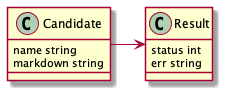
\includegraphics[width=8cm]{candidate}
            \caption{후보 클래스 다이어그램}
        \end{center}
    \end{figure}

    \subsubsection{후보 등록}

    후보 등록은 클라이언트와 별도의 앱에서 수행된다. 관리자 앱에서 후보의 이름과 마크다운을 입력 받으면 Candidate 구조체를 만들어 서버에 전송한다. 서버는 전송받은 후보 정보가 voters 데이터베이스에 존재하는 지 확인하고 존재하면 에러 상태를 반환하고 존재하지 않으면 후보를 데이터베이스에 저장한다.

    \subsubsection{후보 삭제}

    후보 삭제는 위의 Candidate 클래스에서 이름만 입력하여 사용한다. HTTP DELETE 요청을 /candidate/:name에 요청하면 서버는 받은 데이터를 기반으로 후보가 있는 지 확인하고 삭제한다.

    \subsubsection{후보 수정}

    후보 수정은 후보 등록과 거의 동일하게 동작한다. 대신 후보 등록 때는 있으면 에러, 없으면 등록이었지만 수정은 있으면 수정, 없으면 에러를 반환한다.

\subsection{서버 관리자 설문조사 구현}

\subsection{옵저버 구현}

    \subsubsection{}

\newpage
\section{부록}

    \begin{figure}[h]
        \begin{center}
            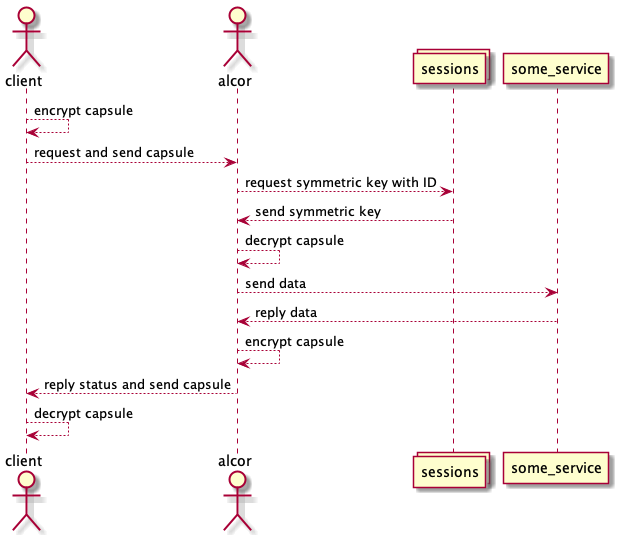
\includegraphics[width=14cm]{sessions}
            \caption{세션 시퀸스 다이어그램}
        \end{center}
    \end{figure}

    \begin{figure}[h]
        \begin{center}
            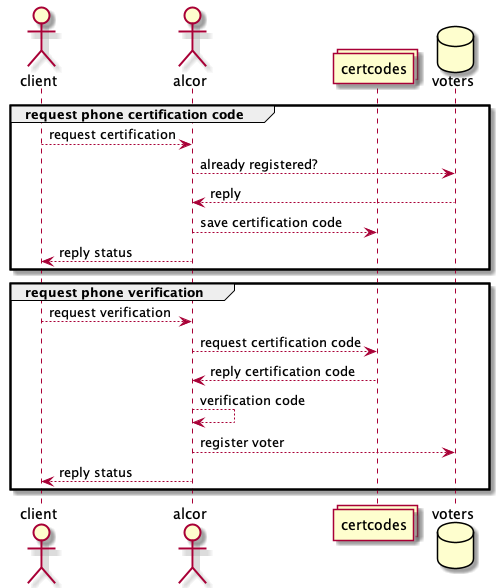
\includegraphics[width=14cm]{client-register}
            \caption{유권자 등록 시퀸스 다이어그램}
        \end{center}
    \end{figure}

    \begin{figure}[h]
        \begin{center}
            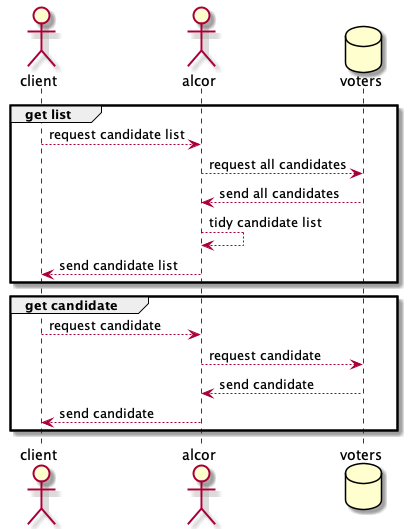
\includegraphics[width=14cm]{candidate-getlist}
            \caption{후보 조회 시퀸스 다이어그램}
        \end{center}
    \end{figure}

    \begin{figure}[h]
        \begin{center}
            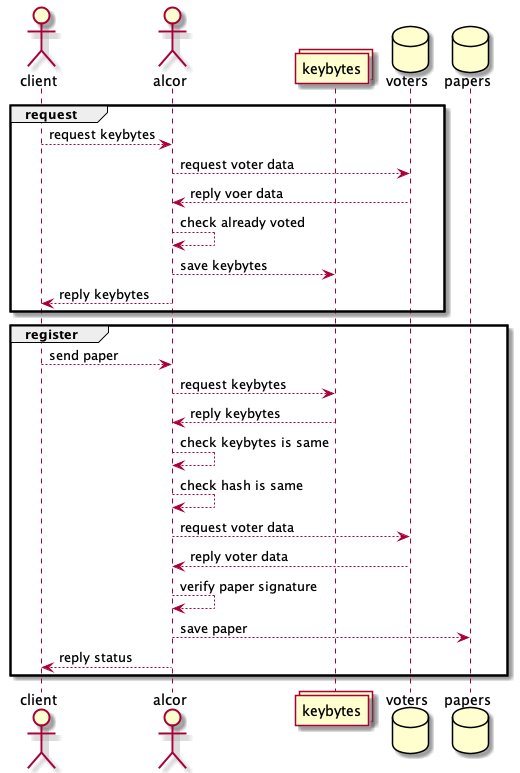
\includegraphics[height=16cm]{vote}
            \caption{투표 시퀸스 다이어그램}
        \end{center}
    \end{figure}

    \begin{figure}[h]
        \begin{center}
            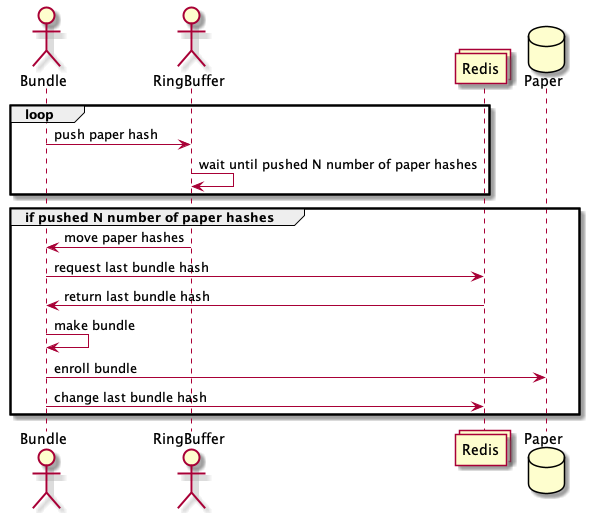
\includegraphics[width=15cm]{bundle-seq}
            \caption{번들 시퀸스 다이어그램}
        \end{center}
    \end{figure}

    \begin{figure}[h]
        \begin{center}
            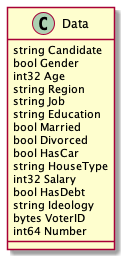
\includegraphics[width=8cm]{survey-class}
            \caption{설문조사 클래스 다이어그램}
        \end{center}
    \end{figure}

    \begin{figure}[h]
        \begin{center}
            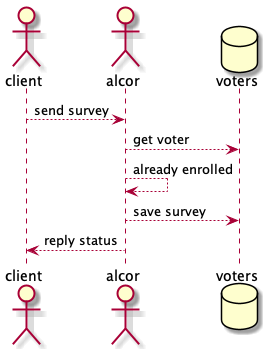
\includegraphics[width=10cm]{survey-seq}
            \caption{설문조사 시퀸스 다이어그램}
        \end{center}
    \end{figure}

    \begin{figure}[h]
        \begin{center}
            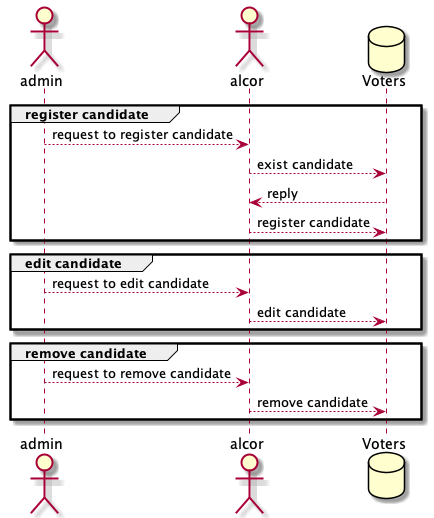
\includegraphics[width=15cm]{candidate-reg}
            \caption{후보 시퀸스 다이어그램}
        \end{center}
    \end{figure}

    \begin{figure}[h]
        \begin{center}
            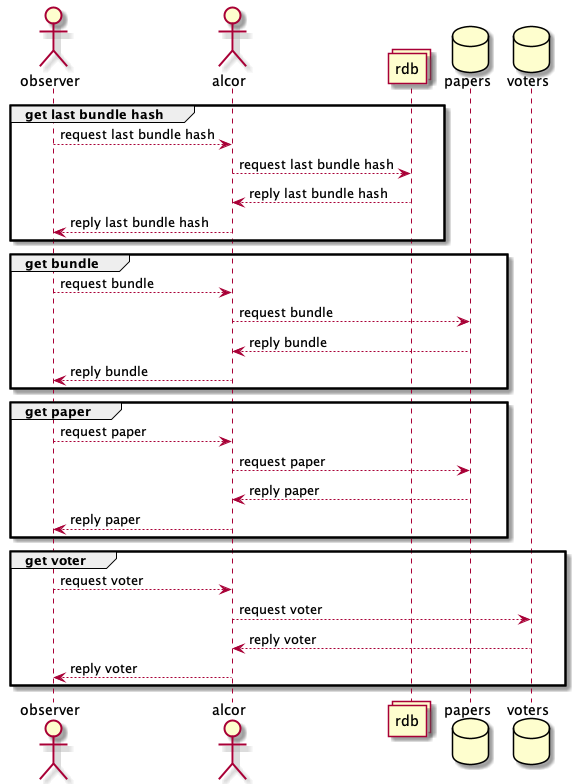
\includegraphics[width=13cm]{observer-get.png}
            \caption{후보 시퀸스 다이어그램}
        \end{center}
    \end{figure}

    \begin{figure}[h]
        \begin{center}
            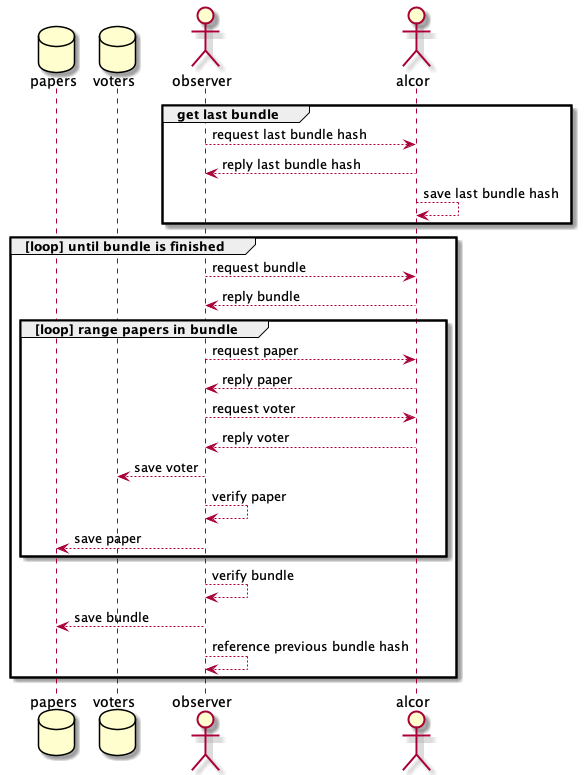
\includegraphics[height=17cm]{observer-verify.png}
            \caption{후보 시퀸스 다이어그램}
        \end{center}
    \end{figure}

\end{document}